\chapter{Projeto dos Componentes da Arquitetura}
\label{sec-componentes}
\vspace{-1cm}

% Permite quebrar melhor os parágrafos com identificadores longos em fonte monoespaçada.
\emergencystretch=3em

Como mostra a Figura~\ref{figura-arquitetura}, o sistema Happy Paws tem três subsistemas: Gestão de Perfis, Serviços e Suporte. Cada um deles é dividido em três camadas: Apresentação, Negócio e Acesso a Dados. Nas seções seguintes, cada subsistema é detalhado, mostrando os modelos de projeto de cada camada.

Na Camada de Negócio, cada subsistema é dividido em dois pacotes, que correspondem às componentes descritas por Falbo~\cite{falbo:notas18}, conforme a Tabela~\ref{tabela-pacotes}: o pacote \texttt{cdp}, com a Componente de Domínio do Problema (CDP), que contém as classes que representam os elementos do domínio e foram identificadas nos modelos estruturais da fase de requisitos; e o pacote \texttt{cgt}, com a Componente de Gerência de Tarefas (CGT), que contém as classes de aplicação (prefixo \texttt{Apl}) que implementam as funcionalidades representadas nas \textit{user stories}. As classes de aplicação são o ponto de entrada da Camada de Negócio e são chamadas pelas \emph{Server Actions} do Next.js, que desempenham o papel de controladoras na Camada de Apresentação.

\begin{footnotesize}
\begin{longtable}{|c|c|}
	\caption{Pacotes da Camada de Negócio e as componentes equivalentes em~\cite{falbo:notas18}.}
	\label{tabela-pacotes}\\\hline
	\rowcolor{lightgray}
	\textbf{Pacote} & \textbf{Componente} \\\hline
	\endfirsthead
	\hline
	\rowcolor{lightgray}
	\textbf{Pacote} & \textbf{Componente} \\\hline
	\endhead
	\texttt{cdp} & Componente de Domínio do Problema (CDP) \\\hline
	\texttt{cgt} & Componente de Gerência de Tarefas (CGT) \\\hline
\end{longtable}
\end{footnotesize}

A Figura~\ref{figura-pacotes} mostra os pacotes da Camada de Negócio e suas dependências. Dentro de cada subsistema, o pacote \texttt{cgt} depende do pacote \texttt{cdp}, que não conhece a aplicação. Entre subsistemas, tanto Serviços quanto Suporte dependem de Gestão de Perfis (seus elementos referenciam Tutor, Passeador, Cachorro, Usuário e Atendente), e Suporte depende também de Serviços, pois um Chamado pode se referir a um Passeio. Além disso, Serviços e Suporte dependem do pacote \texttt{Comum}, que contém a interface \texttt{NotificadorTempoReal}, usada para enviar notificações e eventos em tempo real aos usuários e implementada na infraestrutura do sistema por meio de \textit{Server-Sent Events} (SSE) servidos por \textit{Route Handlers} do Next.js, com o mecanismo LISTEN/NOTIFY do PostgreSQL para repassar os eventos entre instâncias do servidor (RNF-3).

\begin{figure}[h]
	\centering
	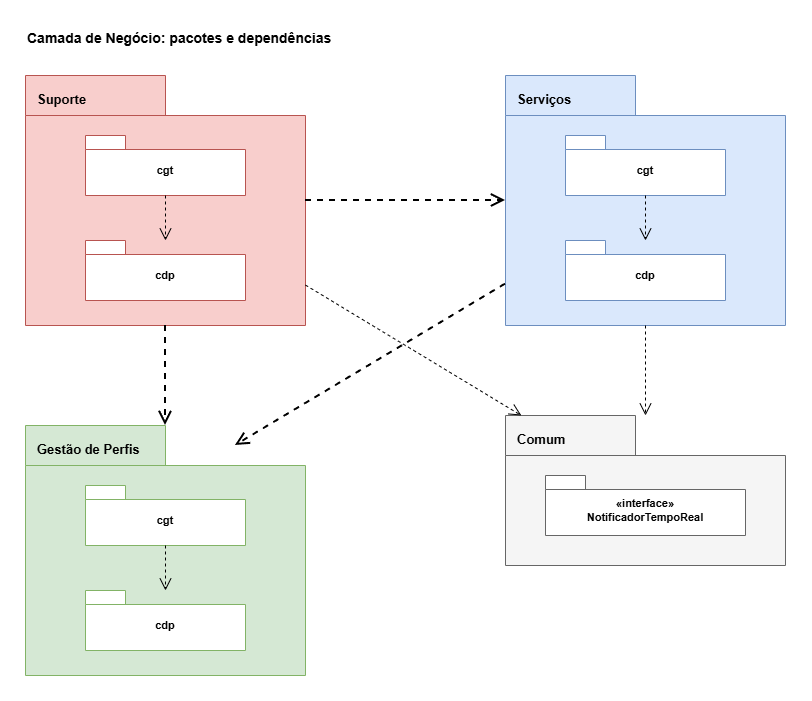
\includegraphics[width=1\textwidth,height=0.7\textheight,keepaspectratio]{figuras/ln-pacotes.png}
	\caption{Pacotes da Camada de Negócio e suas dependências.}
	\label{figura-pacotes}
\end{figure}


%=======================================================================================================
\section{Subsistema Gestão de Perfis}
\label{sec-componentes-perfis}

O subsistema Gestão de Perfis cuida do cadastro de tutores, cães e passeadores. Ele também cuida da validação de identidade dos passeadores e do compartilhamento de perfis de cães entre tutores (US01 a US06).


\subsection{Camada de Negócio}
\label{sec-componentes-perfis-negocio}

A Figura~\ref{figura-perfis-cdp} mostra o projeto da Componente de Domínio do Problema (pacote \texttt{cdp}) do subsistema Gestão de Perfis, obtido a partir do diagrama de classes do Documento de Especificação de Requisitos (Figura 35).

\begin{figure}[h]
	\centering
	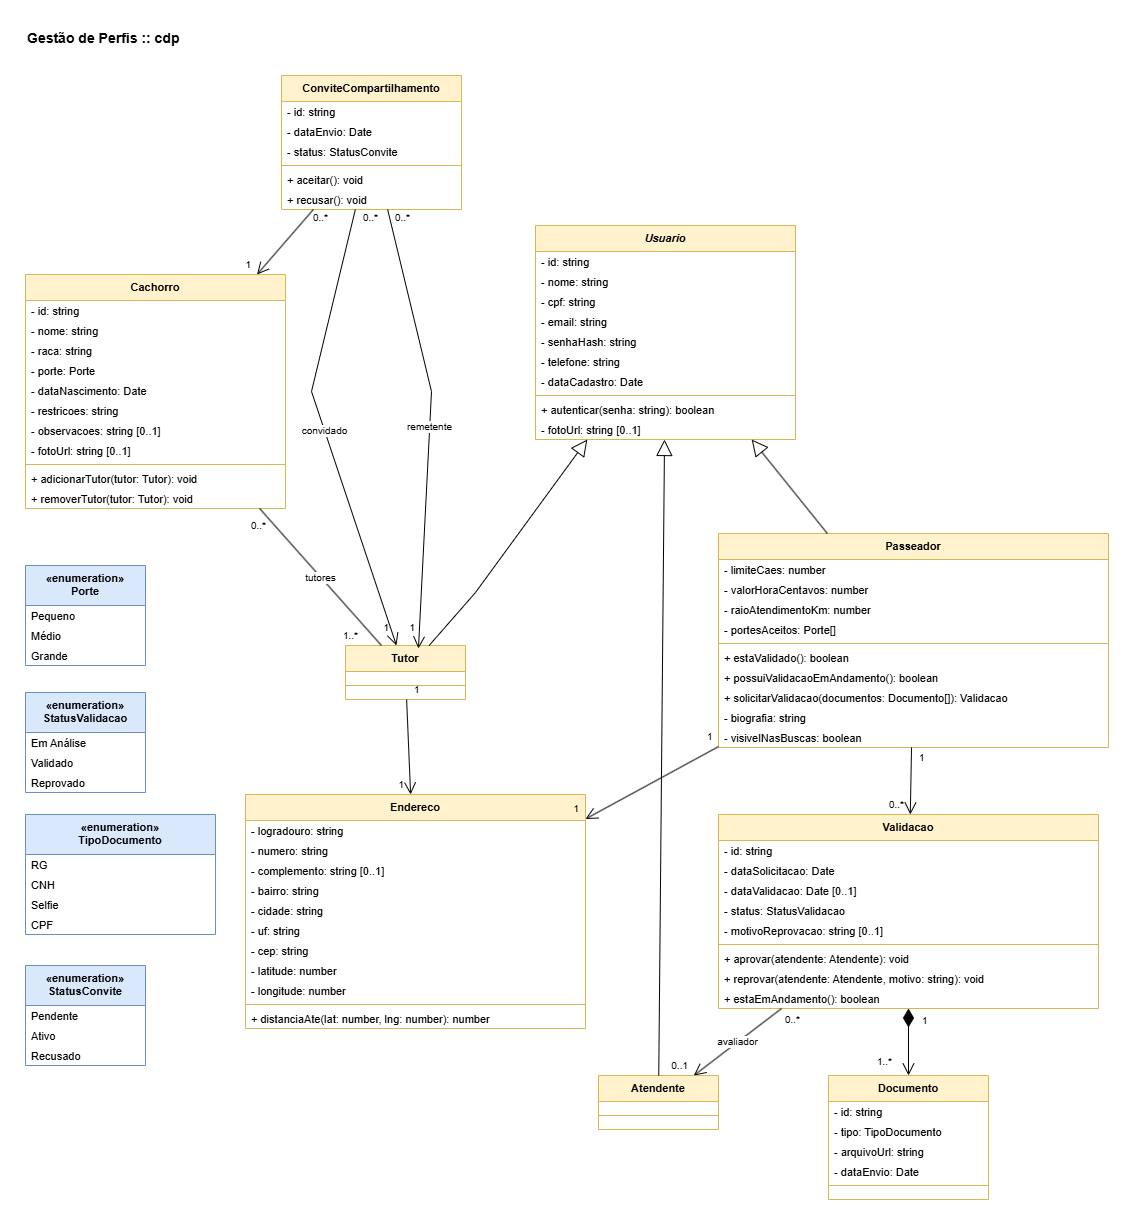
\includegraphics[width=1\textwidth,height=0.85\textheight,keepaspectratio]{figuras/ln-perfis-cdp.png}
	\caption{Projeto da Componente de Domínio do Problema (\texttt{cdp}) do subsistema Gestão de Perfis.}
	\label{figura-perfis-cdp}
\end{figure}

As principais decisões que levaram a este modelo, em relação ao modelo de requisitos, foram:

\begin{itemize}
	\item \textbf{Generalização de Pessoa em Usuário.} A classe abstrata \texttt{Pessoa} do modelo de requisitos foi renomeada para \texttt{Usuario}, generalizando Tutor, Passeador e Atendente. Foram acrescentados \texttt{senhaHash}, \texttt{dataCadastro} e a operação \texttt{autenticar()}, necessários para o acesso ao sistema, e o atributo \texttt{fotoUrl}, que corresponde à foto de perfil das telas de cadastro. A autenticação é feita pela biblioteca Better Auth (Capítulo~\ref{sec-plataforma}): \texttt{senhaHash} e \texttt{autenticar()} representam, no CDP, a credencial do usuário, mas o hash da senha é calculado e guardado pela própria biblioteca, em sua tabela de contas, e a operação \texttt{AplCadastroUsuario.autenticar()} apenas delega a ela a verificação, de modo que o código do sistema nunca calcula nem compara hashes de senha. Como o Drizzle ORM não oferece herança de entidades, a generalização é realizada no banco de dados por uma tabela comum de usuários, referenciada por chave estrangeira pelas tabelas de cada papel.

	\item \textbf{Criação da classe Validação.} No modelo de requisitos, o estado da validação era o atributo \texttt{status} de Passeador, mas as restrições RI-4 (um Passeador não pode ter mais de uma Validação ao mesmo tempo) e RI-5 (a data de envio dos Documentos deve ser anterior ou igual à data de conclusão da Validação) já tratavam a Validação como um conceito próprio. Foi criada, então, a classe \texttt{Validacao}, com os atributos \texttt{dataSolicitacao}, \texttt{dataValidacao}, \texttt{status} e \texttt{motivoReprovacao} (este exigido pelo CA04.4), associada a um Passeador (que passa a ter um histórico de validações), a seus Documentos (composição) e ao Atendente que a avaliou. O \texttt{status} deixou de ser atributo de Passeador, que passa a obter essa informação por meio da operação \texttt{estaValidado()}.

	\item \textbf{Criação da classe ConviteCompartilhamento.} O compartilhamento de perfil de um cão entre tutores (US05) possui estado próprio (pendente até o aceite, ativo depois do aceite, CA05.2 e CA05.3) e envolve três participantes: o cão, o tutor que convida (\texttt{remetente}) e o tutor convidado (\texttt{convidado}). Por isso, foi criada a classe \texttt{ConviteCompartilhamento}, com as operações \texttt{aceitar()} e \texttt{recusar()}. A associação entre Cachorro e Tutor permanece muitos-para-muitos, com a cardinalidade mínima 1 do lado do Tutor, que garante a RI-3.

	\item \textbf{Atributos do Passeador.} Foram acrescentados \texttt{biografia} (CA03.1), \texttt{portesAceitos} (campo ``Porte aceito'' da tela de cadastro, usado como filtro na busca, CA07.1) e \texttt{visivelNasBuscas} (controle de disponibilidade da tela de modo de trabalho, CA06.4). O preço por hora passou a ser armazenado em centavos (\texttt{valorHoraCentavos}), evitando erros de arredondamento com números de ponto flutuante. O atributo \texttt{raioAtendimentoKm} apoia a busca por geolocalização citada no propósito do sistema.

	\item \textbf{Atributos de Endereço e de Cachorro.} Endereço ganhou \texttt{latitude} e \texttt{longitude} e a operação \texttt{distanciaAte()}, que permitem filtrar passeadores por proximidade. Em Cachorro, a idade foi substituída por \texttt{dataNascimento} (a idade é calculada), e foram mantidos \texttt{restricoes} (alergias e medos, CA02.1) e \texttt{observacoes} (campo livre da tela de cadastro).

	\item \textbf{Enumerações.} Os valores das enumerações seguem os nomes dos critérios de aceitação do documento de requisitos: \texttt{StatusValidacao} (Em Análise, Validado, Reprovado), \texttt{StatusConvite} (Pendente, Ativo, Recusado, este último introduzido pela operação \texttt{recusar()}) e \texttt{TipoDocumento} (RG, CNH, Selfie, CPF).
\end{itemize}

A Figura~\ref{figura-perfis-cgt} mostra o projeto da Componente de Gerência de Tarefas (pacote \texttt{cgt}) do subsistema, que depende das classes do pacote \texttt{cdp}. Cada classe de aplicação agrupa as operações de um conjunto de \textit{user stories}:

\begin{figure}[h]
	\centering
	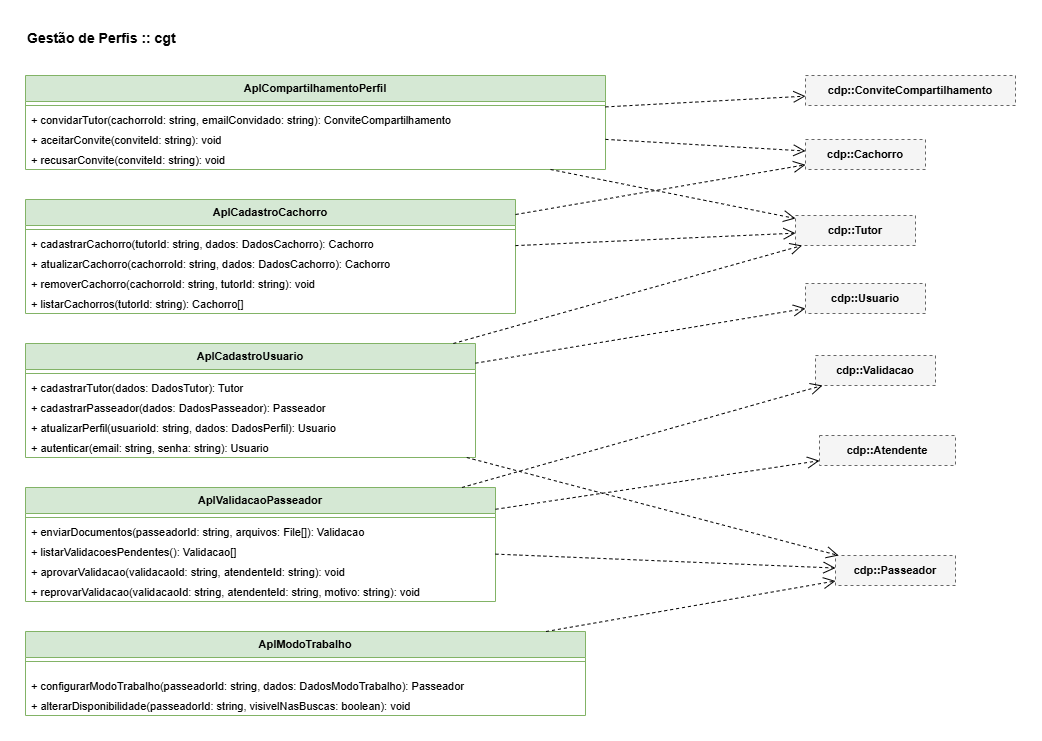
\includegraphics[width=1\textwidth,height=0.85\textheight,keepaspectratio]{figuras/ln-perfis-cgt.png}
	\caption{Projeto da Componente de Gerência de Tarefas (\texttt{cgt}) do subsistema Gestão de Perfis.}
	\label{figura-perfis-cgt}
\end{figure}

\begin{itemize}
	\item \texttt{AplCadastroUsuario}: cadastro de Tutor e de Passeador, atualização de perfil e autenticação (US01, US03). Verifica a unicidade de CPF e e-mail (RI-1 e RI-2);
	\item \texttt{AplCadastroCachorro}: cadastro, atualização, remoção e listagem de cães de um Tutor (US02). Garante que todo Cachorro tenha ao menos um Tutor (RI-3);
	\item \texttt{AplCompartilhamentoPerfil}: envio, aceite e recusa de convites de compartilhamento (US05);
	\item \texttt{AplValidacaoPasseador}: envio de documentos pelo Passeador e aprovação ou reprovação da Validação pelo Atendente (US04). Impede mais de uma Validação em andamento por Passeador (RI-4) e confere as datas dos Documentos (RI-5);
	\item \texttt{AplModoTrabalho}: definição de preço por hora, limite de cães, portes aceitos e disponibilidade do Passeador (US06), rejeitando valores inválidos (CA06.2).
\end{itemize}


\subsection{Camada de Apresentação}
\label{sec-componentes-perfis-apresentacao}

Esta camada tem as telas de cadastro de Tutor e de Passeador, a tela de cadastro de cão, a tela de compartilhamento de perfil de pet e a tela usada pelo Atendente para validar documentos, conforme as telas mostradas nas Figuras 1 a 6 do documento de requisitos.


\subsection{Camada de Acesso a Dados}
\label{sec-componentes-perfis-dados}

\begin{sloppypar}
Esta camada guarda e busca os dados do subsistema no banco PostgreSQL, usando o Drizzle ORM. Ela é formada pelos repositórios: \texttt{TutorRepository}, \texttt{PasseadorRepository}, \texttt{CachorroRepository}, \texttt{EnderecoRepository}, \texttt{ValidacaoRepository}, \texttt{DocumentoRepository} e \texttt{ConviteCompartilhamento\-Repository}, que seguem as classes do \texttt{cdp} apresentado na Figura~\ref{figura-perfis-cdp}.
\end{sloppypar}



%=======================================================================================================
\section{Subsistema Serviços}
\label{sec-componentes-servicos}

O subsistema Serviços cuida da busca por passeadores, do agendamento de passeios (avulsos ou fixos), da execução do passeio em tempo real (GPS, alertas e fotos), do pagamento, da avaliação e das conquistas do pet (US07 a US15).


\subsection{Camada de Negócio}
\label{sec-componentes-servicos-negocio}

A Figura~\ref{figura-servicos-cdp} mostra o projeto da Componente de Domínio do Problema do subsistema Serviços, obtido a partir do diagrama de classes do Documento de Especificação de Requisitos (Figura 36). As classes Tutor, Passeador e Cachorro pertencem ao subsistema Gestão de Perfis e são apenas referenciadas.

\begin{figure}[h]
	\centering
	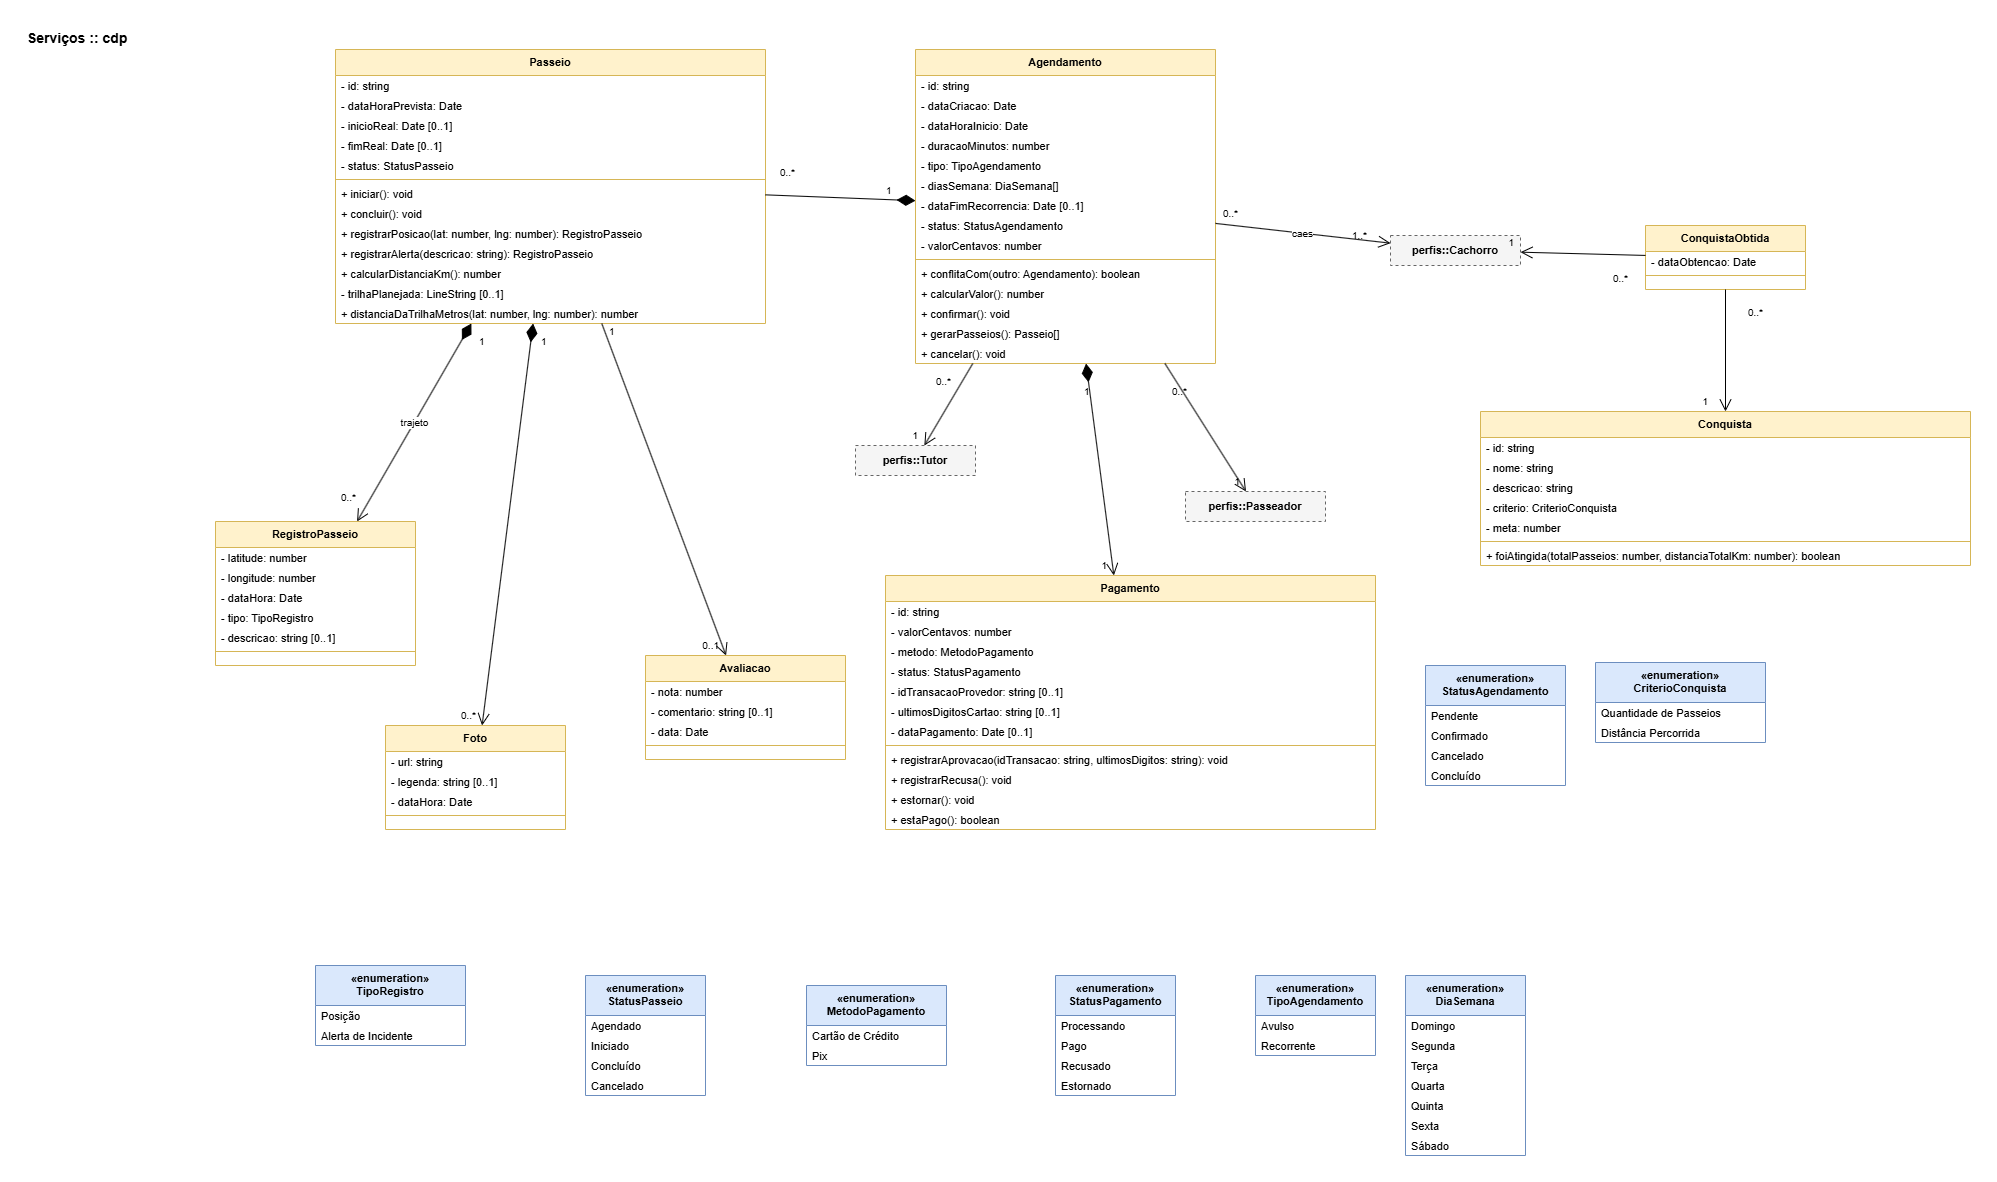
\includegraphics[width=1\textwidth,height=0.85\textheight,keepaspectratio]{figuras/ln-servicos-cdp.png}
	\caption{Projeto da Componente de Domínio do Problema (\texttt{cdp}) do subsistema Serviços.}
	\label{figura-servicos-cdp}
\end{figure}

As principais decisões que levaram a este modelo, em relação ao modelo de requisitos, foram:

\begin{itemize}
	\item \textbf{Agendamento e Passeio.} Um Agendamento recorrente gera vários Passeios (um por ocorrência), por isso a associação é de composição, e os Passeios são criados pela operação \texttt{gerarPasseios()}. A cardinalidade do lado do Passeio é 0..*, pois um Agendamento pendente ainda não possui Passeios. O Agendamento passou a guardar \texttt{dataHoraInicio} (que substitui a data e a hora de início separadas), \texttt{duracaoMinutos}, \texttt{dataFimRecorrencia} (para agendamentos fixos) e \texttt{valorCentavos}, o valor calculado no momento do agendamento. Guardar o valor no Agendamento faz com que alterações posteriores de preço do Passeador só valham para novos contratos (CA06.4).

	\item \textbf{Pagamento associado ao Agendamento.} No modelo de requisitos, o Pagamento aparecia associado ao Passeio, mas a RI-4 (um Agendamento só pode ser confirmado se o Pagamento correspondente estiver pago) e o agendamento recorrente, cobrado mensalmente (Figura 12 do documento de requisitos), mostram que o pagamento se refere ao Agendamento. Em atendimento ao RNF-2, o Pagamento não guarda o número do cartão, apenas o identificador da transação no provedor (\texttt{idTransacaoProvedor}) e os últimos dígitos (\texttt{ultimosDigitosCartao}). A enumeração \texttt{StatusPagamento} tem os valores Processando, Pago, Recusado (CA14.2 a CA14.4) e Estornado, que permite desfazer um pagamento quando o Agendamento é cancelado.

	\item \textbf{Estado do Passeio.} A enumeração \texttt{StatusPasseio} foi redefinida como Agendado, Iniciado, Concluído e Cancelado, que são os estados citados nos critérios de aceitação (CA10.1, CA11.1, CA11.2), em lugar de Realizado e Em\_Andamento. O Passeio passou a ter \texttt{dataHoraPrevista}, \texttt{inicioReal} e \texttt{fimReal} e as operações \texttt{iniciar()}, \texttt{concluir()} e \texttt{calcularDistanciaKm()}.

	\item \textbf{Trilha planejada e desvio de rota.} O modelo de requisitos cita uma ``trilha pré-definida'' (CA10.3), mas não possui user story para cadastrar trilhas. Por isso, a trilha não foi modelada como classe: ela é um dado opcional do Passeio, o atributo \texttt{trilhaPlanejada}, que guarda a linha (sequência de coordenadas) informada ao agendar ou ao iniciar o passeio. A operação \texttt{distanciaDaTrilhaMetros()} calcula a distância de uma posição à trilha, e a classe \texttt{AplExecucaoPasseio} usa esse valor, a cada posição registrada por \texttt{registrarPosicao()}, para detectar o desvio de mais de 100 metros e avisar o tutor por meio de \texttt{NotificadorTempoReal}, o que faz o trajeto aparecer em vermelho. Quando o Passeio não tem trilha planejada, essa verificação não se aplica.

	\item \textbf{Registro do trajeto e alertas.} Como o alerta de incidente do Passeador (minimundo) e o trajeto de GPS são ambos registros ocorridos durante o Passeio, a classe RegistroPasseio recebeu o atributo \texttt{tipo} (Posição ou Alerta de Incidente) e o atributo opcional \texttt{descricao}.

	\item \textbf{Fotos e mural.} A classe Foto é composta pelo Passeio. O mural de um cão (US13) é obtido pelos Passeios dos Agendamentos que o incluem, o que dispensa a associação direta entre Cachorro e Foto do modelo de requisitos.

	\item \textbf{Conquistas.} A classe Conquista do modelo de requisitos foi dividida em duas: \texttt{Conquista}, que define o marco (\texttt{criterio} e \texttt{meta}, por exemplo, 50 km percorridos) e a operação \texttt{foiAtingida()}, e \texttt{ConquistaObtida}, que registra a data em que um Cachorro obteve uma Conquista. Assim, a definição da conquista não é repetida para cada cão.

	\item \textbf{Comentário da Avaliação.} O atributo \texttt{comentario} de Avaliação é opcional (0..1), enquanto a \texttt{nota} é obrigatória (de 1 a 5). O documento de requisitos é inconsistente nesse ponto: o CA15.2 exige nota e comentário, mas a tela de avaliação (Figura 24) marca o comentário como opcional. Prevaleceu a tela, para não impedir que o Tutor avalie um passeio apenas com a nota; a descrição do CA15.2 deve ser ajustada no documento de requisitos para refletir essa decisão.

	\item \textbf{Alertas durante o passeio.} A perda de sinal de GPS por mais de 2 minutos (CA10.4) e o atraso de mais de 15 minutos no encerramento (CA11.3 e CA11.4) não exigiram novas classes nem atributos, pois podem ser calculados a partir de dados já persistidos. A perda de sinal é a diferença entre a hora atual e a \texttt{dataHora} do último \texttt{RegistroPasseio} de um Passeio iniciado. O atraso é a hora atual ultrapassar em mais de 15 minutos a soma de \texttt{dataHoraPrevista} do Passeio com a \texttt{duracaoMinutos} do Agendamento. Uma tarefa periódica do servidor (por exemplo, uma rota acionada por um agendador do ambiente de hospedagem) consulta os Passeios com status ``Iniciado'', aplica essas duas regras e avisa o Tutor por meio de \texttt{NotificadorTempoReal}, o mesmo usado por \texttt{AplExecucaoPasseio}. O cronômetro em vermelho da tela do Passeador (CA11.3) é um comportamento da Camada de Apresentação, que compara a hora atual com o horário previsto de término. Esses alertas são eventos transitórios, não persistidos.

	\item \textbf{Enumerações.} \texttt{TipoAgendamento} (Avulso, Recorrente), \texttt{StatusAgendamento} (Pendente, Confirmado, Cancelado, Concluído), \texttt{DiaSemana}, \texttt{MetodoPagamento} (Cartão de Crédito, Pix), \texttt{CriterioConquista} e \texttt{TipoRegistro}.
\end{itemize}

A Figura~\ref{figura-servicos-cgt} mostra o projeto da Componente de Gerência de Tarefas do subsistema Serviços, e as classes de aplicação são:

\begin{figure}[h]
	\centering
	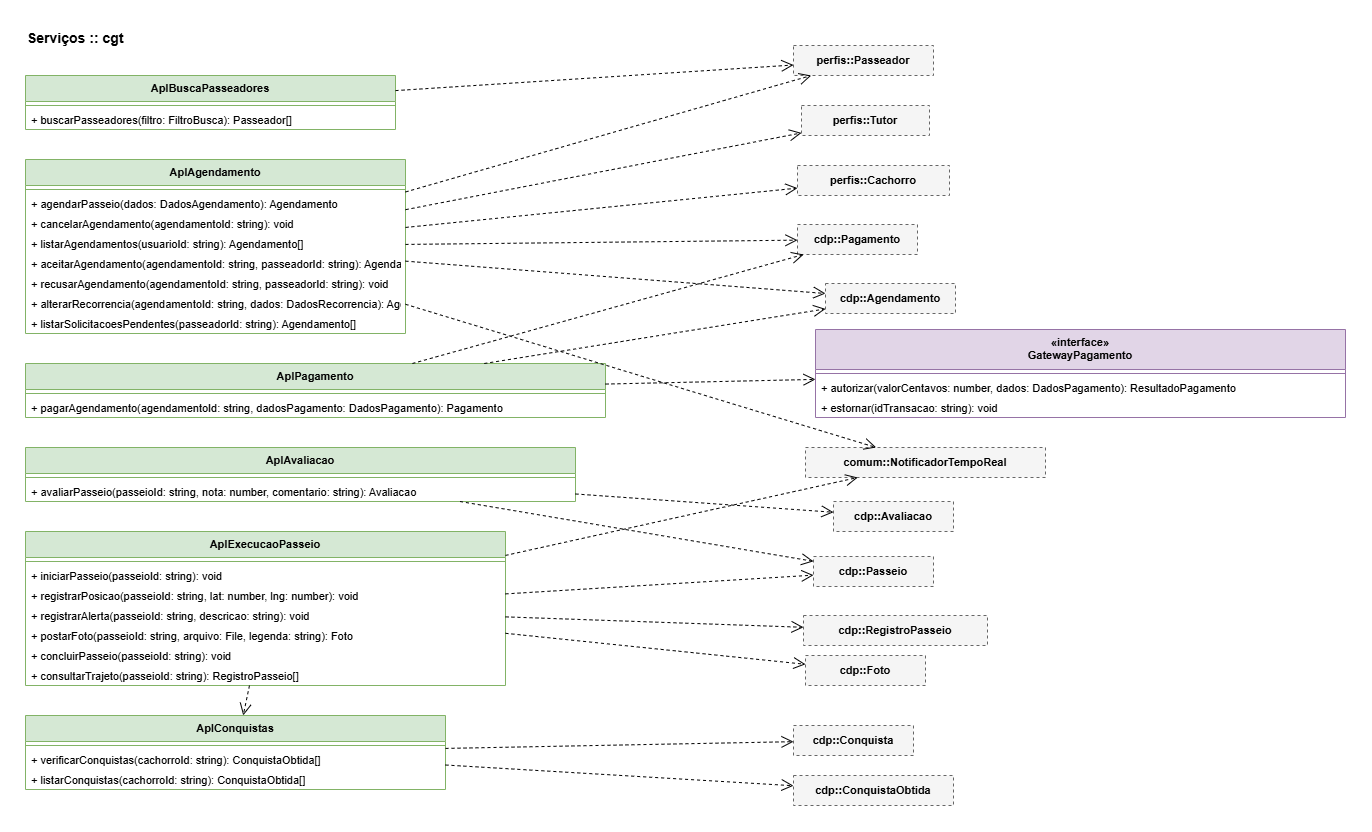
\includegraphics[width=1\textwidth,height=0.85\textheight,keepaspectratio]{figuras/ln-servicos-cgt.png}
	\caption{Projeto da Componente de Gerência de Tarefas (\texttt{cgt}) do subsistema Serviços.}
	\label{figura-servicos-cgt}
\end{figure}

\begin{itemize}
	\item \texttt{AplBuscaPasseadores}: busca de passeadores por filtros (US07);
	\item \texttt{AplAgendamento}: criação de agendamentos avulsos e recorrentes, cancelamento e listagem (US08, US09), além de aceite e recusa pelo Passeador, alteração de recorrência e listagem das solicitações pendentes (CA08.4, CA09.4, CA09.5). Verifica as restrições RI-1, RI-5 e RI-6 e notifica o Tutor por meio de \texttt{NotificadorTempoReal};
	\item \texttt{AplPagamento}: pagamento de um Agendamento (US14), por meio da interface \texttt{GatewayPagamento}, que isola o provedor de pagamento externo;
	\item \texttt{AplExecucaoPasseio}: início, registro de posições e alertas, postagem de fotos, consulta do trajeto e conclusão do Passeio (US10 a US12), publicando os eventos em tempo real por meio de \texttt{NotificadorTempoReal} e acionando \texttt{AplConquistas} na conclusão. Garante que o início real do Passeio não anteceda a data do Agendamento (RI-2) e que o fim real não anteceda o início real (RI-3);
	\item \texttt{AplAvaliacao}: avaliação do Passeio concluído pelo Tutor (US15);
	\item \texttt{AplConquistas}: verificação e listagem das conquistas de um Cachorro (US13).
\end{itemize}

A Figura~\ref{figura-servicos-seq-agendar} detalha o fluxo da operação \texttt{agendarPasseio}. A página de agendamento chama \texttt{AplAgendamento.agendarPasseio()}, que busca o Tutor, o Passeador e os Cachorros nos repositórios e verifica se o Passeador está validado e visível nas buscas. Em seguida, cria o Agendamento, cujo construtor recusa um início anterior à data de criação (RI-1), busca os agendamentos ativos do Passeador e do Cachorro no horário, verifica a existência de conflito para cada um deles (RI-5) e confere se a soma de cães respeita o \texttt{limiteCaes} do Passeador (RI-6). Por fim, calcula o valor, cria o Pagamento associado, salva o Agendamento e exibe a tela de pagamento.

\begin{figure}[h]
	\centering
	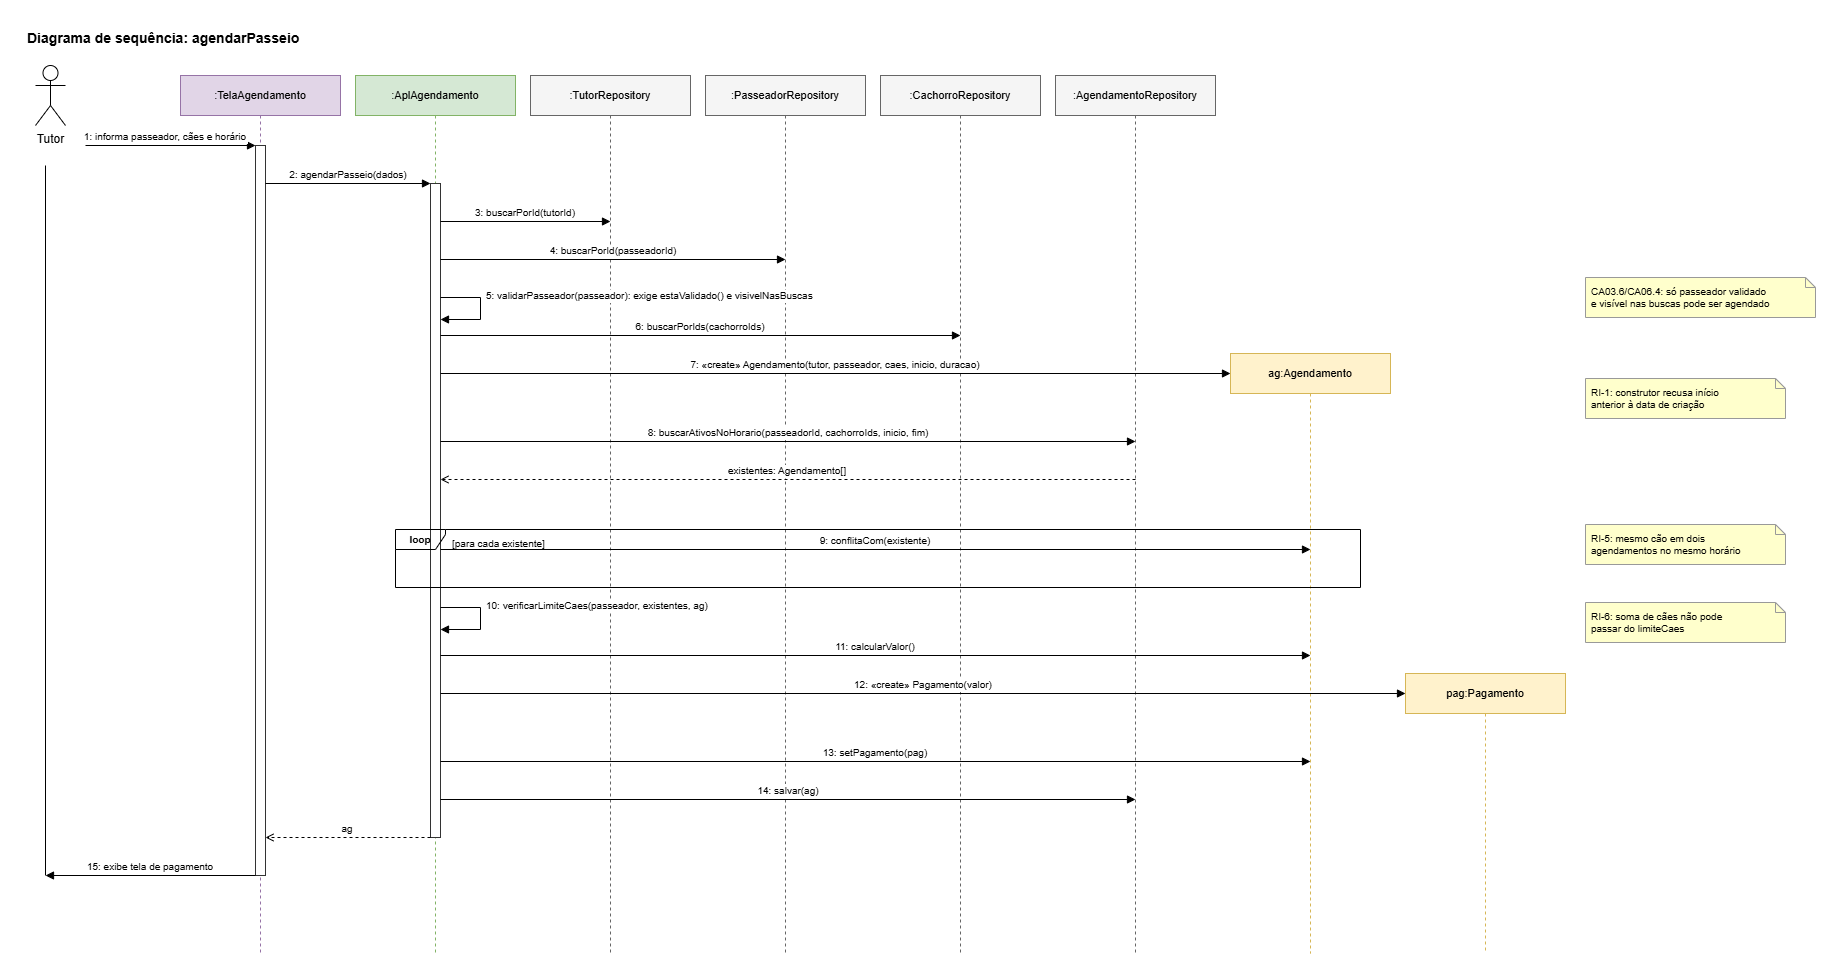
\includegraphics[width=1\textwidth,height=0.85\textheight,keepaspectratio]{figuras/ln-servicos-seq-agendar.png}
	\caption{Diagrama de sequência da operação \texttt{agendarPasseio}.}
	\label{figura-servicos-seq-agendar}
\end{figure}

O pagamento é solicitado logo após a criação do Agendamento. O Agendamento nasce com status ``Pendente'' e o Pagamento com status ``Processando''. Quando o Pagamento é confirmado (``Pago'') e o Passeador aceita a solicitação, o Agendamento passa a ``Confirmado'' (RI-4, CA08.4 e CA09.4). Se o Passeador recusa a solicitação ou o Tutor cancela o Agendamento, o Pagamento é estornado (``Estornado''). Essa escolha prevalece sobre a frase do minimundo que prevê o pagamento após o trajeto, por ser compatível com a RI-4 e com o CA14.5, que impede o início de um Passeio sem pagamento confirmado.


\subsection{Camada de Apresentação}
\label{sec-componentes-servicos-apresentacao}

Esta camada tem as telas de busca de passeadores, de agendamento (avulso e fixo), de acompanhamento do trajeto pelo GPS, de postagem de fotos, de pagamento e de avaliação do passeio, conforme as telas mostradas nas Figuras 7 a 24 do documento de requisitos.


\subsection{Camada de Acesso a Dados}
\label{sec-componentes-servicos-dados}

\begin{sloppypar}
Esta camada guarda e busca os dados do subsistema no banco, usando o Drizzle ORM. Ela é formada pelos repositórios: \texttt{AgendamentoRepository}, \texttt{PasseioRepository}, \texttt{RegistroPasseioRepository}, \texttt{PagamentoRepository}, \texttt{AvaliacaoRepository}, \texttt{FotoRepository}, \texttt{ConquistaRepository} e \texttt{ConquistaObtidaRepository}, que seguem as classes do \texttt{cdp} apresentado na Figura~\ref{figura-servicos-cdp}.
\end{sloppypar}



%=======================================================================================================
\section{Subsistema Suporte}
\label{sec-componentes-suporte}

O subsistema Suporte cuida dos chamados abertos por Tutores ou Passeadores e do atendimento feito pelos Atendentes (US16 e US17).


\subsection{Camada de Negócio}
\label{sec-componentes-suporte-negocio}

A Figura~\ref{figura-suporte-cdp} mostra o projeto da Componente de Domínio do Problema do subsistema Suporte, obtido a partir do diagrama de classes do Documento de Especificação de Requisitos (Figura 37).

\begin{figure}[h]
	\centering
	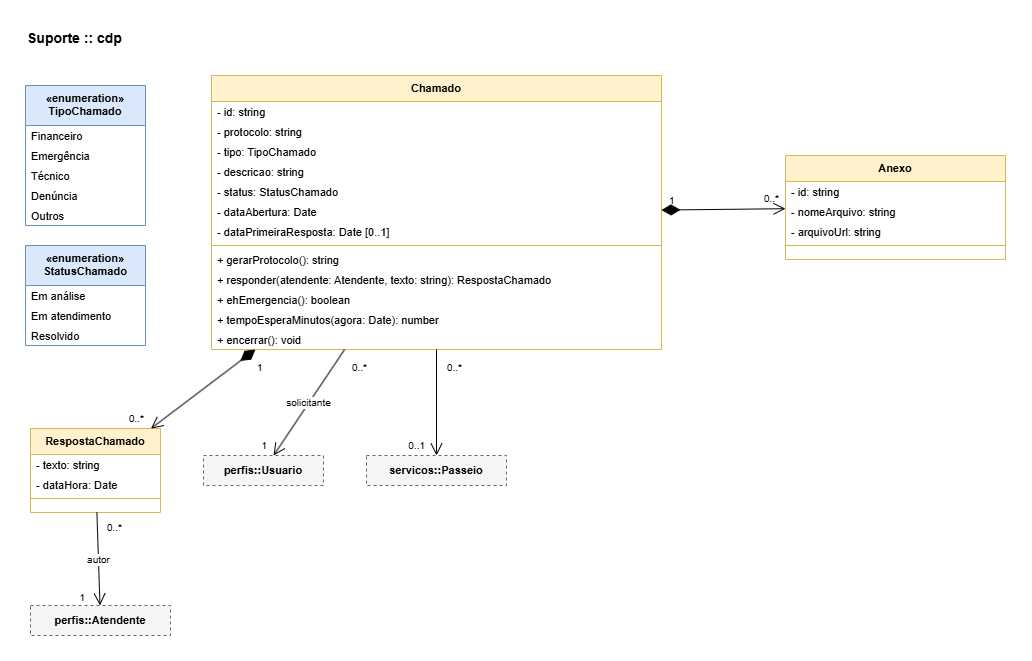
\includegraphics[width=1\textwidth,height=0.8\textheight,keepaspectratio]{figuras/ln-suporte-cdp.png}
	\caption{Projeto da Componente de Domínio do Problema (\texttt{cdp}) do subsistema Suporte.}
	\label{figura-suporte-cdp}
\end{figure}

As principais decisões que levaram a este modelo, em relação ao modelo de requisitos, foram:

\begin{itemize}
	\item \textbf{Solicitante do Chamado.} As duas associações ``abre'', de Tutor e de Passeador, foram substituídas por uma única associação \texttt{solicitante} com a classe Usuário, de Gestão de Perfis.
	\item \textbf{Criação da classe RespostaChamado.} O CA17.5 exige o registro do horário de cada interação do Atendente, e o CA17.4 exige a mudança de status na primeira resposta. Foi criada a classe \texttt{RespostaChamado} (texto e data/hora), composta pelo Chamado e com o Atendente como autor, que substitui a associação ``atende''. O atributo \texttt{dataPrimeiraResposta} em Chamado permite calcular o tempo de primeiro atendimento do RNF-4.
	\item \textbf{Criação da classe Anexo.} O CA17.3 exige que o Atendente visualize ou baixe as fotos e capturas de tela anexadas pelo usuário, o que o modelo de requisitos não representava. Foi criada a classe \texttt{Anexo}, composta pelo Chamado.
	\item \textbf{Chamado e Passeio.} Um Chamado pode se referir opcionalmente a um Passeio (por exemplo, um passeador que não apareceu). Essa associação cria a dependência de Suporte em relação a Serviços mostrada na Figura~\ref{figura-pacotes}.
	\item \textbf{Atributos do Chamado.} O \texttt{protocolo} passou a ser uma \textit{string}, já que os protocolos exibidos nas telas têm letras (por exemplo, EMG-2024-002), e \texttt{dataAbertura} substitui \texttt{data}. As operações \texttt{ehEmergencia()} e \texttt{tempoEsperaMinutos()} apoiam a priorização e o tempo de espera exibidos ao Atendente (CA17.1 e CA17.2).
	\item \textbf{Enumerações.} \texttt{TipoChamado} (Financeiro, Emergência, Técnico, Denúncia, Outros), conforme o CA16.1, e \texttt{StatusChamado} (Em análise, Em atendimento, Resolvido).
\end{itemize}

A Figura~\ref{figura-suporte-cgt} mostra o projeto da Componente de Gerência de Tarefas do subsistema Suporte, e as classes de aplicação são:

\begin{figure}[h]
	\centering
	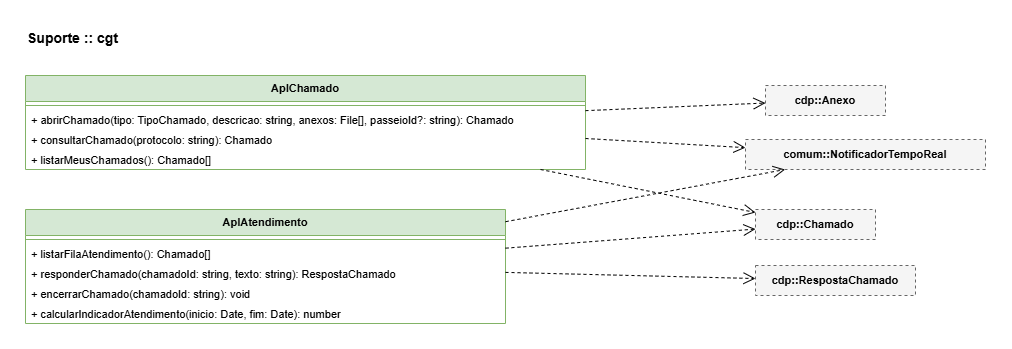
\includegraphics[width=1\textwidth,height=0.7\textheight,keepaspectratio]{figuras/ln-suporte-cgt.png}
	\caption{Projeto da Componente de Gerência de Tarefas (\texttt{cgt}) do subsistema Suporte.}
	\label{figura-suporte-cgt}
\end{figure}

\begin{itemize}
	\item \texttt{AplChamado}: abertura de chamado com tipo, descrição e anexos, consulta por protocolo e listagem dos chamados do usuário (US16). Exige o tipo e a descrição do problema (CA16.1), gera o protocolo e define o status inicial como ``Em análise'' (CA16.2);
	\item \texttt{AplAtendimento}: listagem da fila de atendimento com os chamados de emergência no topo, resposta e encerramento de chamados (US17), e cálculo do indicador de tempo de primeiro atendimento (RNF-4). Ao responder, muda o status para ``Em atendimento'' e notifica o usuário por meio de \texttt{NotificadorTempoReal} (CA16.3).
\end{itemize}


\subsection{Camada de Apresentação}
\label{sec-componentes-suporte-apresentacao}

Esta camada tem a tela de abertura de chamado, usada por Tutores e Passeadores, e as telas da central de atendimento, usadas pelo Atendente, conforme as telas mostradas nas Figuras 25 a 30 do documento de requisitos.


\subsection{Camada de Acesso a Dados}
\label{sec-componentes-suporte-dados}

Esta camada guarda e busca os dados do subsistema no banco, usando o Drizzle ORM. Ela é formada pelos repositórios \texttt{ChamadoRepository}, \texttt{RespostaChamadoRepository} e \texttt{AnexoRepository}, que seguem as classes do \texttt{cdp} apresentado na Figura~\ref{figura-suporte-cdp}.